\documentclass[a4paper, 12pt]{article}

\usepackage[utf8]{inputenc}
\usepackage[spanish]{babel}
\usepackage[margin=1.5in]{geometry}
\usepackage{graphicx}
\usepackage{float}
\usepackage{pdfpages}
\usepackage{listings}
\usepackage{listingsutf8}
\usepackage{xcolor}
\usepackage{scrextend}
\usepackage{array, multirow}
\usepackage{booktabs}
\usepackage{tabularx}

\definecolor{mGreen}{rgb}{0,0.6,0}
\definecolor{mGray}{rgb}{0.5,0.5,0.5}
\definecolor{mPurple}{rgb}{0.58,0,0.82}
\definecolor{backgroundColour}{rgb}{0.95,0.95,0.92}

\newcolumntype{C}[1]{>{\centering\arraybackslash}p{#1}}

\lstset{
language=C,
%backgroundcolor=\color{backgroundColour},   
commentstyle=\color{mGreen},
%keywordstyle=\color{magenta},
keywordstyle=\color{blue},
%numberstyle=\tiny\color{mGray},
stringstyle=\color{mPurple},
tabsize=4,
basicstyle=\fontsize{11}{13}\ttfamily\footnotesize,
showspaces=false,
showstringspaces=false,
captionpos=b,
breaklines=true
}


%\lstdefinestyle{CStyle}{
%    backgroundcolor=\color{backgroundColour},   
%    commentstyle=\color{mGreen},
%    keywordstyle=\color{magenta},
%    numberstyle=\tiny\color{mGray},
%    stringstyle=\color{mPurple},
%    basicstyle=\footnotesize,
%    breakatwhitespace=false,         
%    breaklines=true,                 
%    captionpos=b,                    
%    keepspaces=true,                 
%    numbers=left,                    
%    numbersep=5pt,                  
%    showspaces=false,                
%    showstringspaces=false,
%    showtabs=false,                  
%    tabsize=2,
%    language=C
%}


\title{		\textbf{Trabajo Práctico 2}\\
			\textbf{Memorias caché}
			}

\author{	Lucas Medrano, \textit{Padrón Nro. 99247}                     	\\
            \texttt{ lucasmedrano97@gmail.com }                           		\\
            Federico Álvarez, \textit{Padrón Nro. 99266}                 	\\
            \texttt{ fede.alvarez1997@gmail.com }                                 	\\[2.5ex]
            \normalsize{Grupo Nro. \quad - 2do. Cuatrimestre de 2018}      	\\
            \normalsize{66.20 Organización de Computadoras}               	\\
            \normalsize{Facultad de Ingeniería, Universidad de Buenos Aires}\\
       }
\date{}

\begin{document}
	\lstset{inputencoding=utf8/latin1} % Incorpora acentos en los listings
	\maketitle
	\thispagestyle{empty}
	\begin{abstract}
		En este trabajo se busca implementar en el lenguaje de programación C un tipo de dato que pueda simular el funcionamiento de una memoria caché de 4KB de capacidad, asociativa por conjuntos de cuatro vías, con política de reemplazo LRU y política de escritura Write Back/Write Allocate, junto con la memoria principal asociada. El objetivo de esta simulación será observar y documentar su comportamiento, para una mejor comprensión de dicho funcionamiento.
	\end{abstract}
	
	\pagebreak
	\thispagestyle{empty}
	\tableofcontents
	\newpage
	
	\setcounter{page}{1}
	
	\section{Desarrollo}
	Para interactuar con la memoria caché se desarrollará un programa capaz de leer de un archivo que contendrá instrucciones de lectura y escritura en una posición de memoria, y un comando para obtener el \textit{miss rate}. Éste recibirá como parámetro el nombre del archivo que contiene las instrucciones a ser ejecutadas.
	\subsection{Implementación}
	\subsubsection{Programa}
	El programa tomará como único parámetro del nombre del archivo y, en caso de que no exista, imprimirá por pantalla un mensaje de error acorde.
	
	Ante cada escritura se mostrará un mensaje indicando si se pudo realizar, y ante cada lectura se mostrará el valor leído.
	En el caso de que una línea del archivo contenga texto que no se corresponde con ninguno de los comandos especificados, simplemente se la ignorará y pasará a la siguiente. Sin embargo, en caso de que la instrucción sea válida pero la dirección o el valor a escribir no, se imprimirá un mensaje por pantalla.
	
	\subsubsection{Memoria caché}
	La estructura de la memoria caché constará de dos subpartes principales, los \textit{sets} y los \textit{bloques}. Cada set contendrá cuatro bloques, y los bloques, ademas de los datos a almacenar en memoria, contendrán toda la metadata necesaria para realizar las tareas de lectura, escritura, reemplazo y \textit{write back}. Todas las posiciones de memoria se inicializarán a \texttt{0}, y se asume que tanto las direcciones como los valores contenidos en ellas no pueden ser negativos.
	
	Por otra parte, habrá también una memoria principal del tamaño especificado que interactuará con el caché cuando sea necesario. Cabe aclarar que será la estructura del caché la que decidirá qué bloque reemplazar cuando un set esté lleno, mediante un seguimiento del bloque menos recientemente utilizado, y cuándo escribir los contenidos de dicho bloque en memoria, mediante un chequeo al bit \textit{dirty}.
	
	Llevará cuenta, además, de la cantidad de misses ocurridos, y de accesos a memoria totales, para presentar así el miss rate.  
	\section{Mediciones}
	A continuación se muestran las salidas y tiempos de corrida de los cinco archivos de prueba. Cabe aclarar que las operaciones de escritura consumen más tiempo ya que requieren del procesamiento de un parámetro extra.
	
	Al correr el programa con el archivo \texttt{prueba.mem} se observa la siguiente salida.
	\begin{verbatim}
	$./cache prueba1.mem
	El valor 255 se escribio correctamente
	El valor 254 se escribio correctamente
	El valor 248 se escribio correctamente
	El valor 96 se escribio correctamente
	El valor 192 se escribio correctamente
	Read 255
	Read 254
	Read 248
	Read 192
	Miss rate: 88%
	\end{verbatim}
	El miss rate obtenido es del 88\%, ya que en ocho de los nueve accesos a memoria se produce un \textit{miss}. Esto se debe a que todas las direcciones ingresadas mapean al mismo set, y con la política de reemplazo LRU, se van reemplazando una a una.
	
	A su vez, utilizando el comando \texttt{time} de la consola, se observa el siguiente tiempo. 
	
	\begin{verbatim}
	real	0m0,003s
	\end{verbatim}
	Cabe destacar que las instrucciones de este archivo implican que además de cargar en el caché el bloque correspondiente, se debe escribir el contenido del bloque reemplazado en memoria, lo que consume más tiempo.
	
	Al ingresar ahora el archivo \texttt{prueba.mem}, se observa el siguiente miss rate, junto con el siguiente tiempo. 
	\begin{verbatim}
	$ time ./cache prueba2.mem
	Read 0
	Read 0
	El valor 10 se escribio correctamente
	Read 10
	El valor 20 se escribio correctamente
	Read 20
	Miss rate: 33%
	
	real	0m0,001s
	\end{verbatim}
	Lo cual es consisente, ya que no sólo se registran menos misses, sino que también se leen menos instrucciones y no se escribe ningún bloque en la memoria principal.
	
	En el caso de \texttt{prueba3.mem}:
	\begin{verbatim}
	$ time ./cache prueba3.mem
	El valor 1 se escribio correctamente
	El valor 2 se escribio correctamente
	El valor 3 se escribio correctamente
	El valor 4 se escribio correctamente
	Read 0
	Read 0
	Read 0
	Read 0
	Read 1
	Read 2
	Read 3
	Read 4
	Miss rate: 50%
	
	real	0m0,002s
	\end{verbatim}
	Se registra un tiempo mayor al de la prueba anterior, que se condice tanto con el mayor porcentaje de misses registrado, como con la mayor cantidad de instrucciones presentes.
	
	Para la prueba 4:
	\begin{verbatim}
	$ time ./cache prueba4.mem
	El valor 256 no es valido
	El valor 2 se escribio correctamente
	El valor 3 se escribio correctamente
	El valor 4 se escribio correctamente
	El valor 5 se escribio correctamente
	Read 0
	Read 2
	Read 3
	Read 4
	Read 5
	Read 0
	Read 0
	Read 0
	Read 2
	Read 3
	Read 4
	Read 5
	Miss rate: 18%
	
	real	0m0,002s
	\end{verbatim}
	En este caso se obtiene un tiempo similar al anterior, lo que se explica observando la gran cantidad de instruccuiones ejecutadas con tan bajo porcentaje de misses, y teniendo en cuenta que los valores inválidos no se procesan y tampoco se deben realizar ni reemplazos ni escrituras de bloques en memoria.
	
	Por último, al correr \texttt{prueba5.mem} se registra:
	\begin{verbatim}
	$ time ./cache prueba5.mem
	La direccion 131072 no es valida
	Read 0
	Read 0
	Read 0
	Read 0
	Read 0
	Miss rate: 60%
	
	real	0m0,001s
	\end{verbatim}
	El tiempo es bajo porque las intrucciones son pocas y la primera instrucción no se procesa.
	
	\section{Conclusiones}
	La realización de este trabajo resultó importante para comprender el funcionamiento de la memoria caché y todas las operaciones involucradas en el proceso de almacenar o leer un dato de memoria. Permitió principalmente visualizar la utilidad de este tipo de estructuras y realizar un profundo seguimiento de las acciones que realiza cada parte por separado. Además fue útil para entender la función de cada uno de los elementos de la metadata contenida en cada bloque, así como del \textit{tag}, \textit{index} y \textit{offset} que componen a la dirección de memoria.
	
		Por último, el desarrollo sirvió para observar en la práctica el funcionamiento de esto, al medir el tiempo de ejecución en cada prueba, observar las diferencias entre estas y relacionarlas con factores como el \textit{miss rate}, la cantidad de reemplazos de bloque realizados, o la cantidad de escritura de bloques en memoria al ser reemplazados.
		
		Se entregan junto con este informe todos los archivos de código fuente y headers que componen el programa.
		
	\newpage
	\section{Apéndice}
	\subsection{Enunciado}

	\begin{figure}[H]
		\centering
		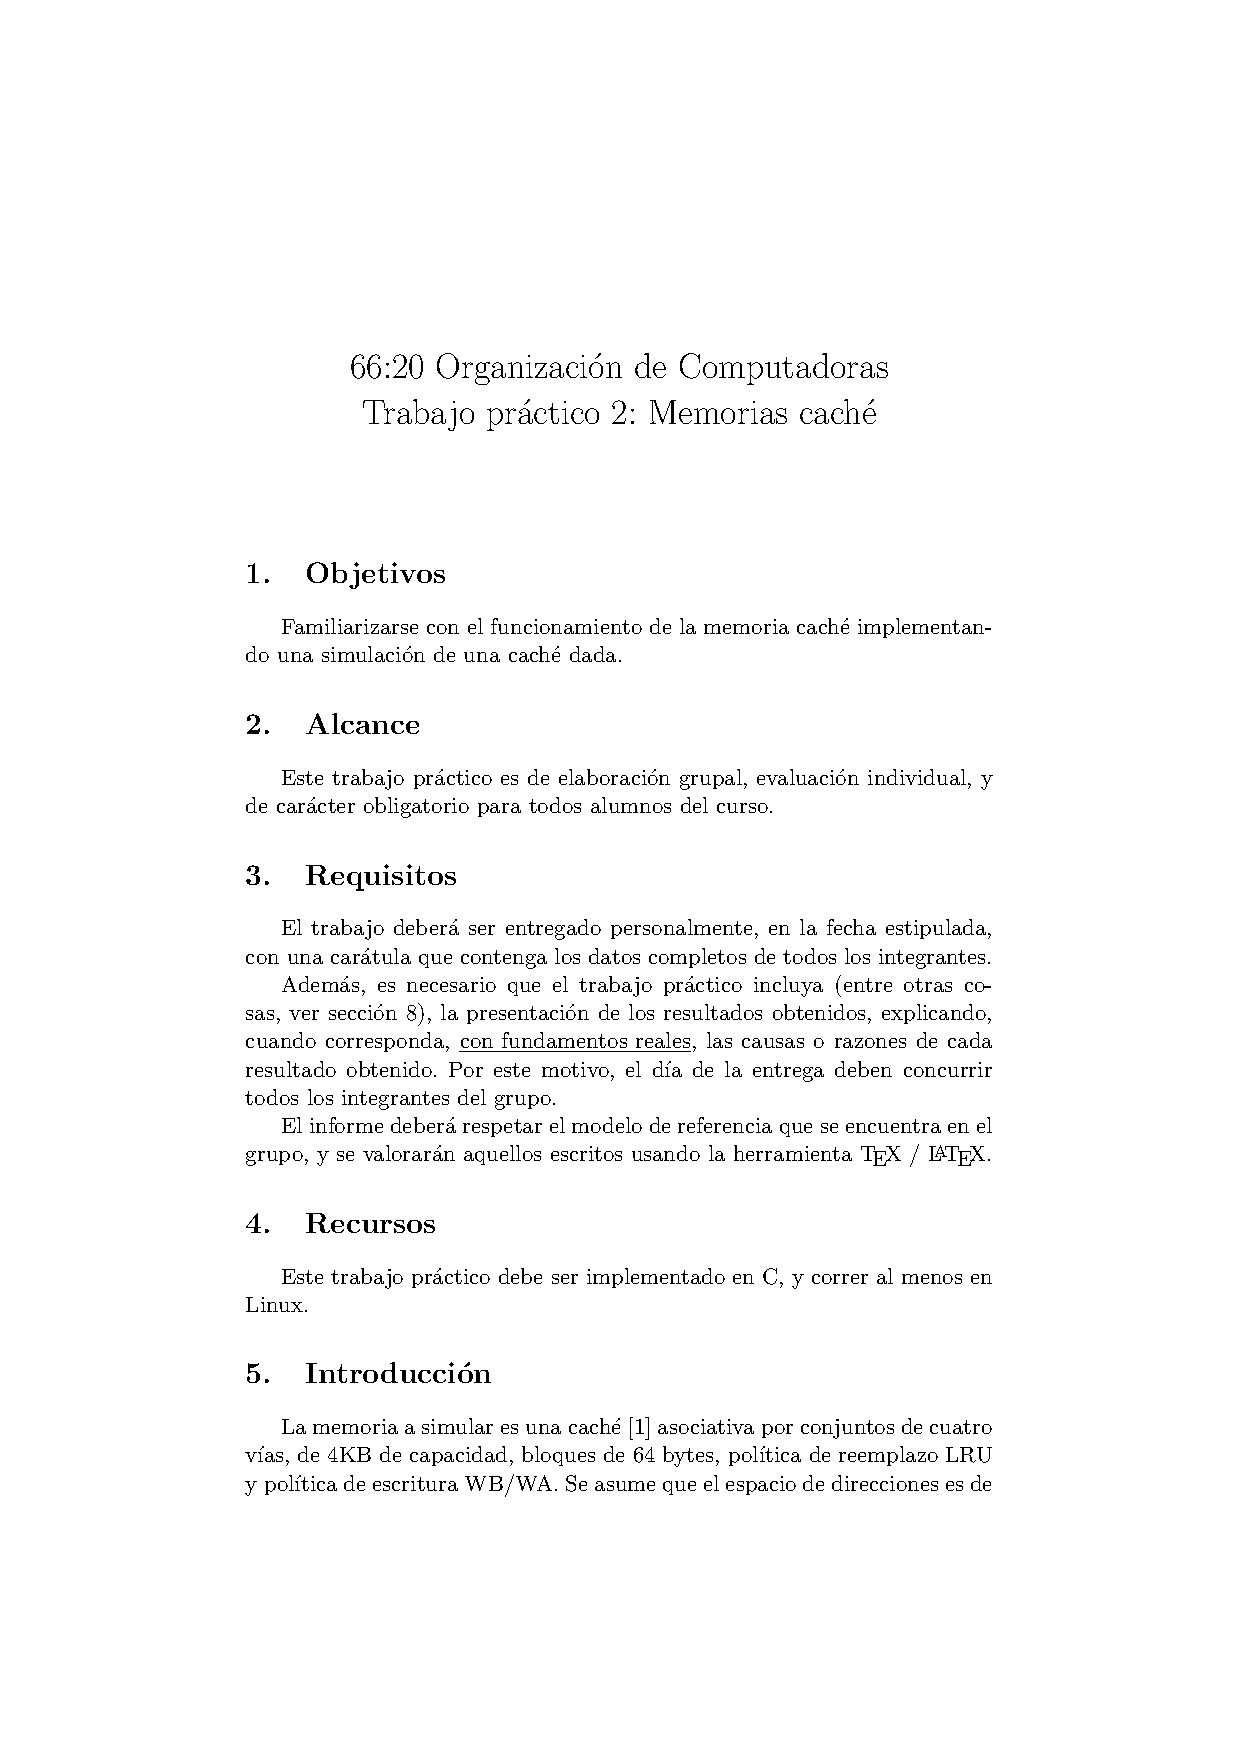
\includegraphics[scale=1, page = 1, clip, trim=1.5in 1.5in 20mm 2in]{files/tp2-c2-2018.pdf}
	\end{figure}
	
	\newpage
	\begin{figure}[H]
		\centering
		\includegraphics[scale=1, page = 2, clip, trim=1.5in 36mm 20mm 1.5in]{files/tp2-c2-2018.pdf}
	\end{figure}
	
	\newpage
	\begin{figure}[H]
		\centering
		\includegraphics[scale=1, page = 3, clip, trim=1.5in 36mm 20mm 1.5in]{files/tp2-c2-2018.pdf}
	\end{figure}
	
	\newpage
	\begin{figure}[H]
		\centering
		\includegraphics[scale=1, page = 4, clip, trim=1.5in 36mm 20mm 1.5in]{files/tp2-c2-2018.pdf}
	\end{figure}
	
\end{document}